%%    _____  _____
%%   |  __ \|  __ \    AUTHOR: Pedro Rivero
%%   | |__) | |__) |   ---------------------------------
%%   |  ___/|  _  /    DATE: November 10, 2021
%%   | |    | | \ \    ---------------------------------
%%   |_|    |_|  \_\   https://github.com/pedrorrivero
%%

\section{QSR}

%% ----------------------------------------------------------------------------
%% ----------------------------------------------------------------------------

\begin{frame}[allowframebreaks]{Algorithm outline}

  \begin{minipage}[c]{\linewidth}
    \begin{center}
      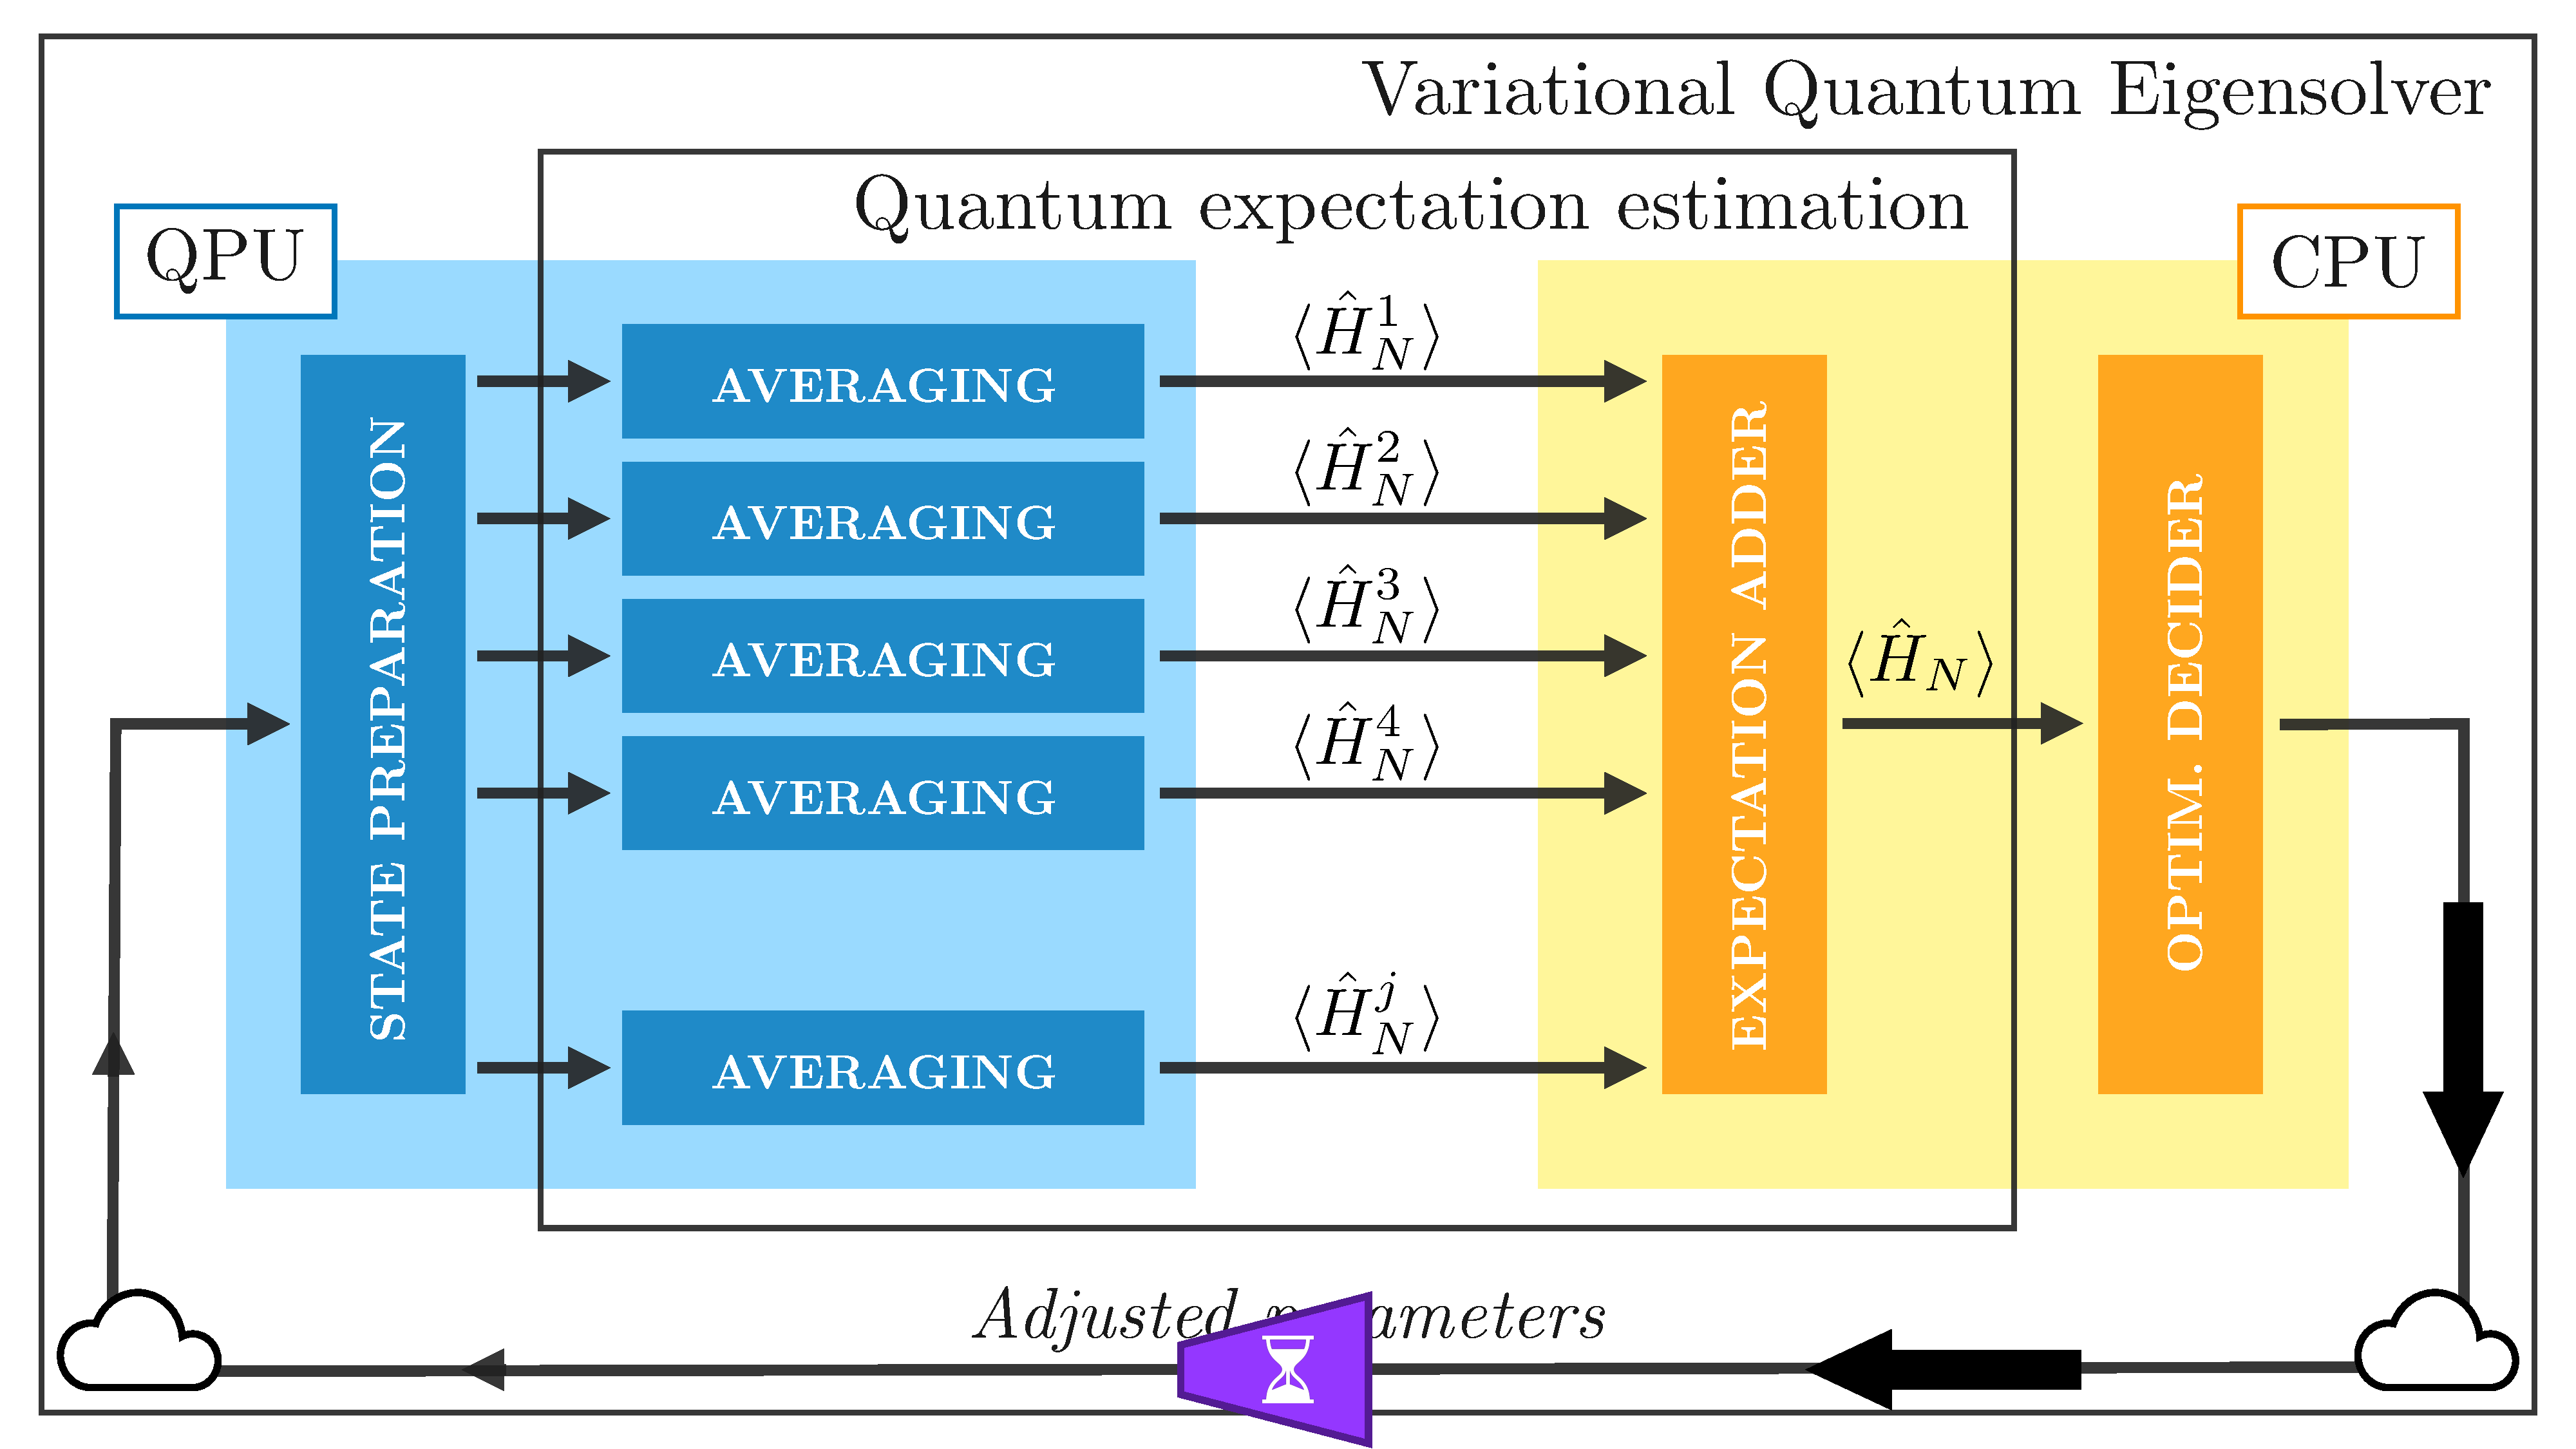
\includegraphics[width=.7\paperwidth]{Figures/VQE-bottleneck}
    \end{center}
  \end{minipage}

%% ----------------------------------------------------------------------------
\break
%% ----------------------------------------------------------------------------

  \begin{minipage}[c]{\linewidth}
    \begin{center}
      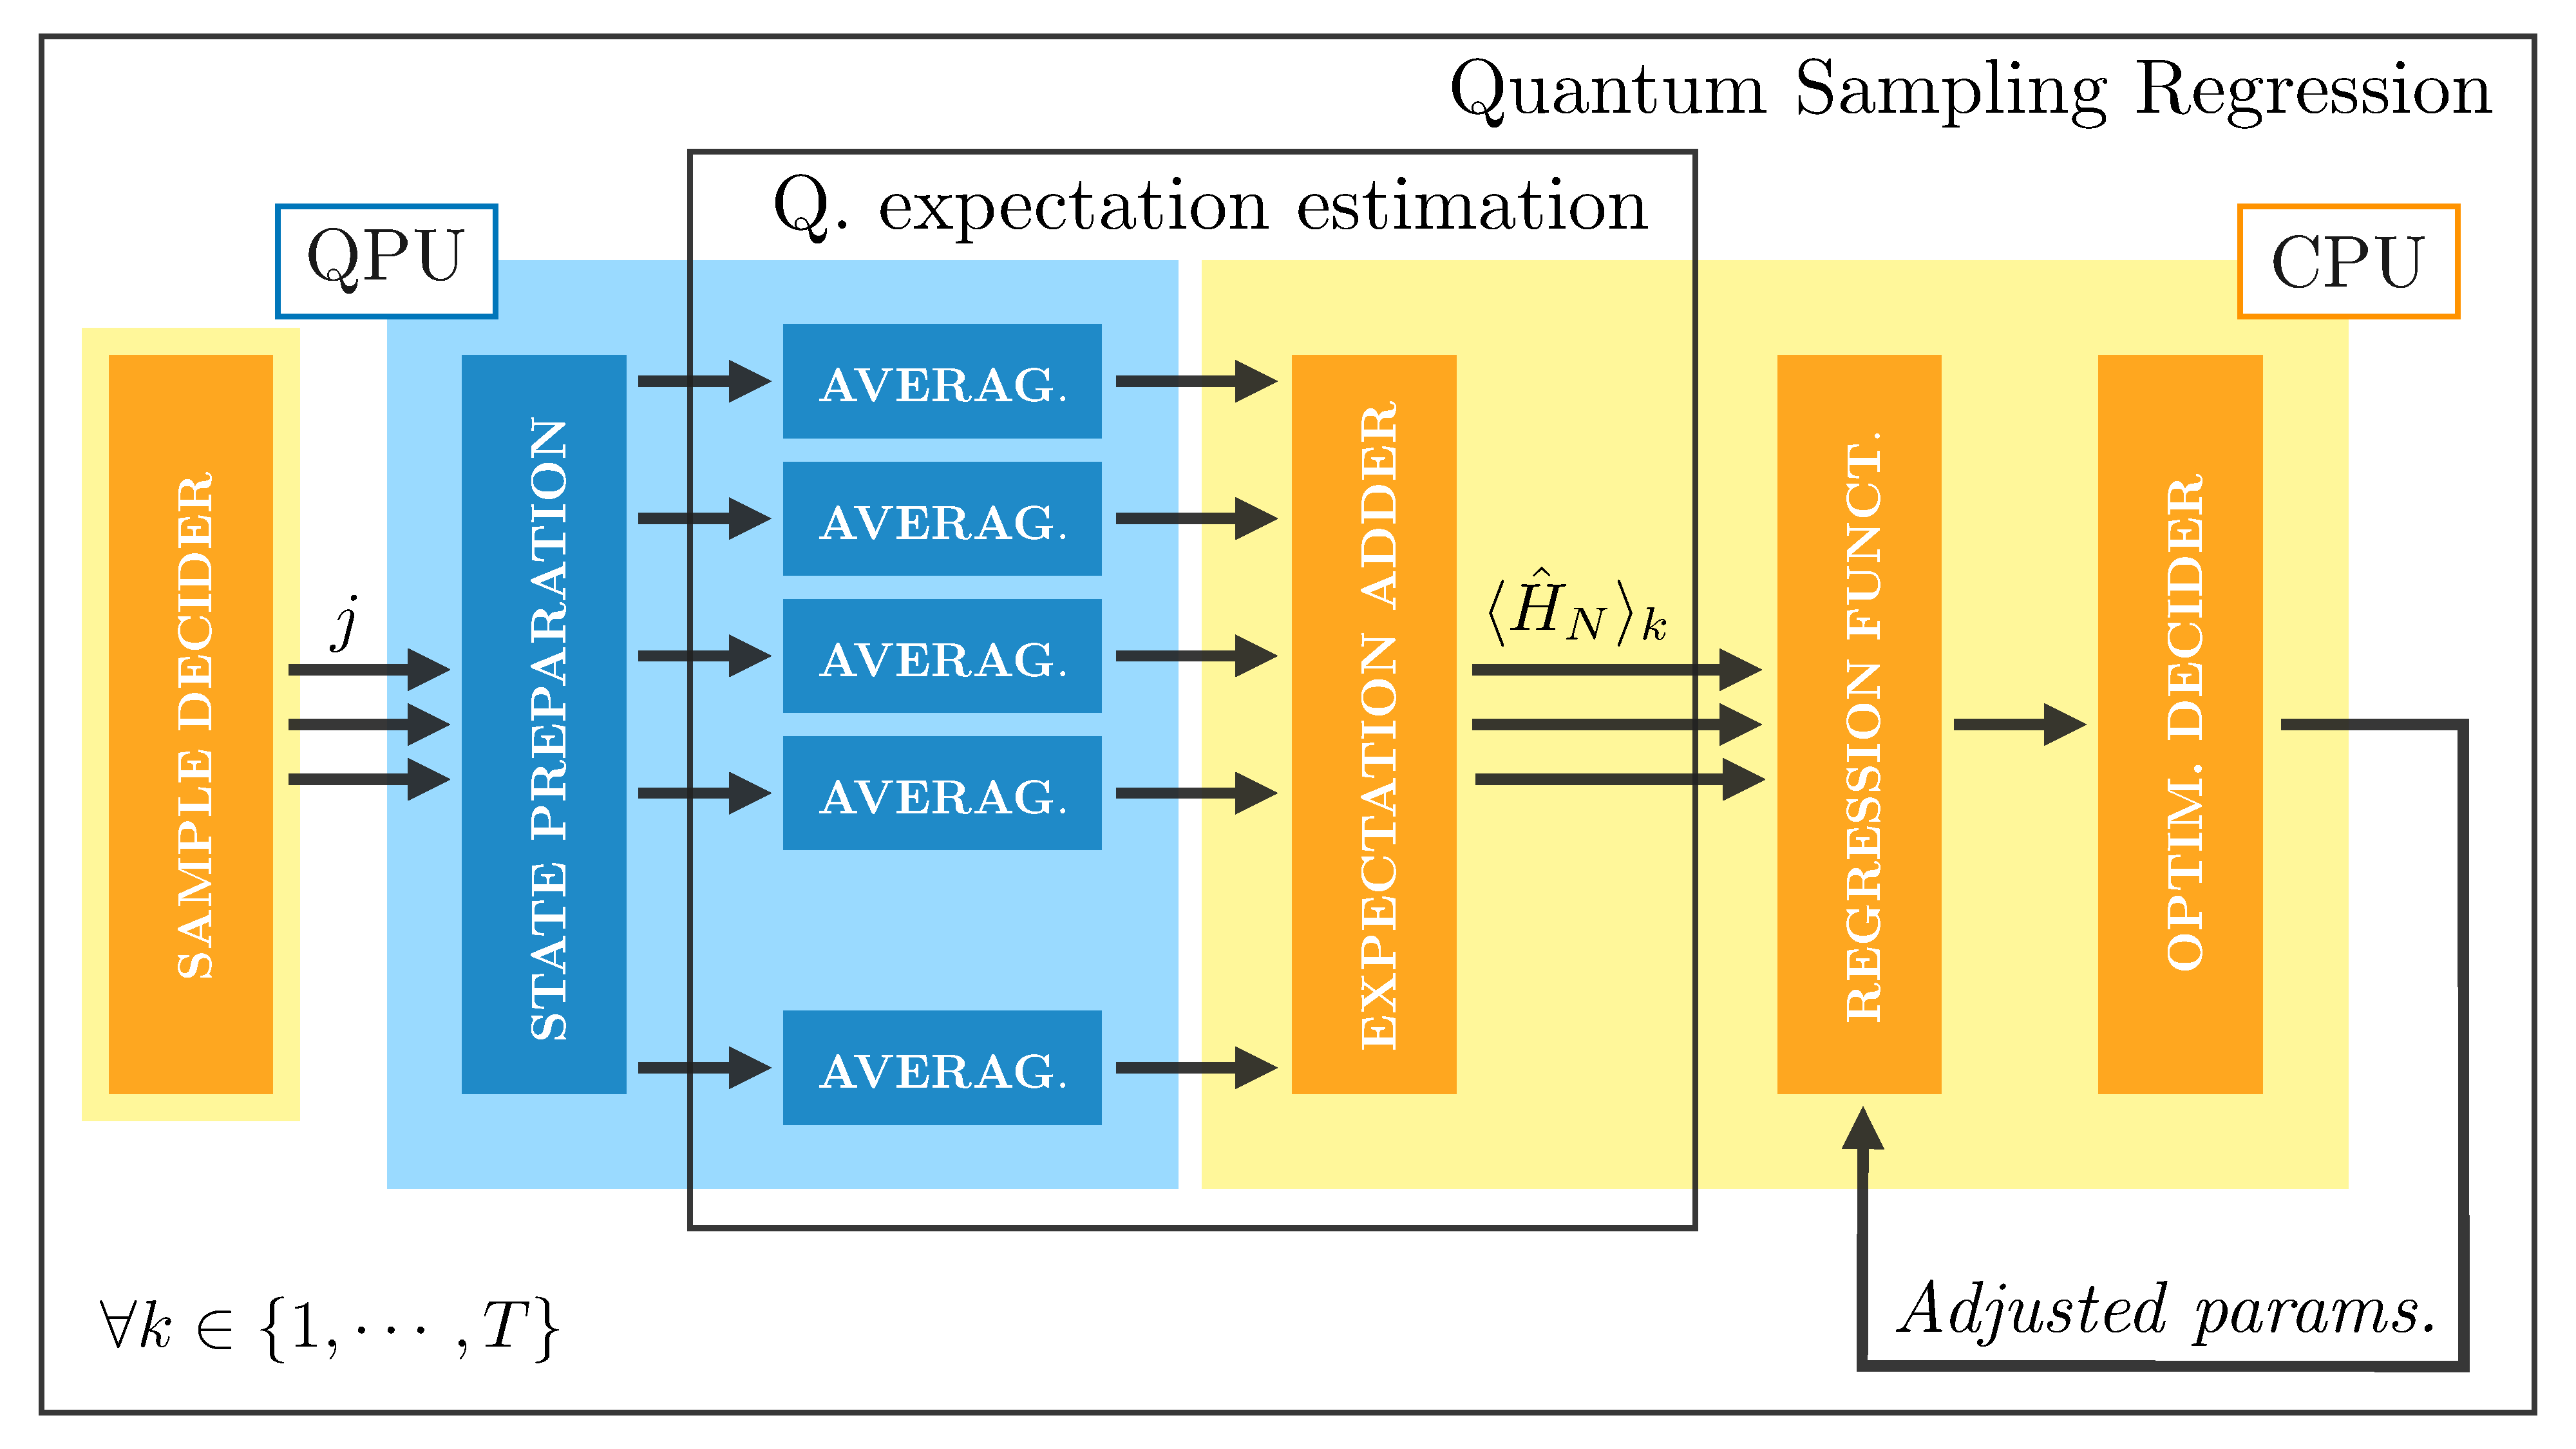
\includegraphics[width=.7\paperwidth]{Figures/chapter05/QSR}
    \end{center}
  \end{minipage}

%% ----------------------------------------------------------------------------
\break
%% ----------------------------------------------------------------------------

  \begin{multicols}{2}

    \begin{itemize}
      \item From the \textbf{topology of the quantum circuit} in charge of state preparation, we can infer a frequency bound.
      \item \textbf{Fourier analysis} then allows to fully reconstruct the expectation value function.
      \item Through the \textbf{Nyquist-Shannon sampling theorem} we can show that our sampling technique is optimal.
    \end{itemize}

    \columnbreak

    \begin{center}
      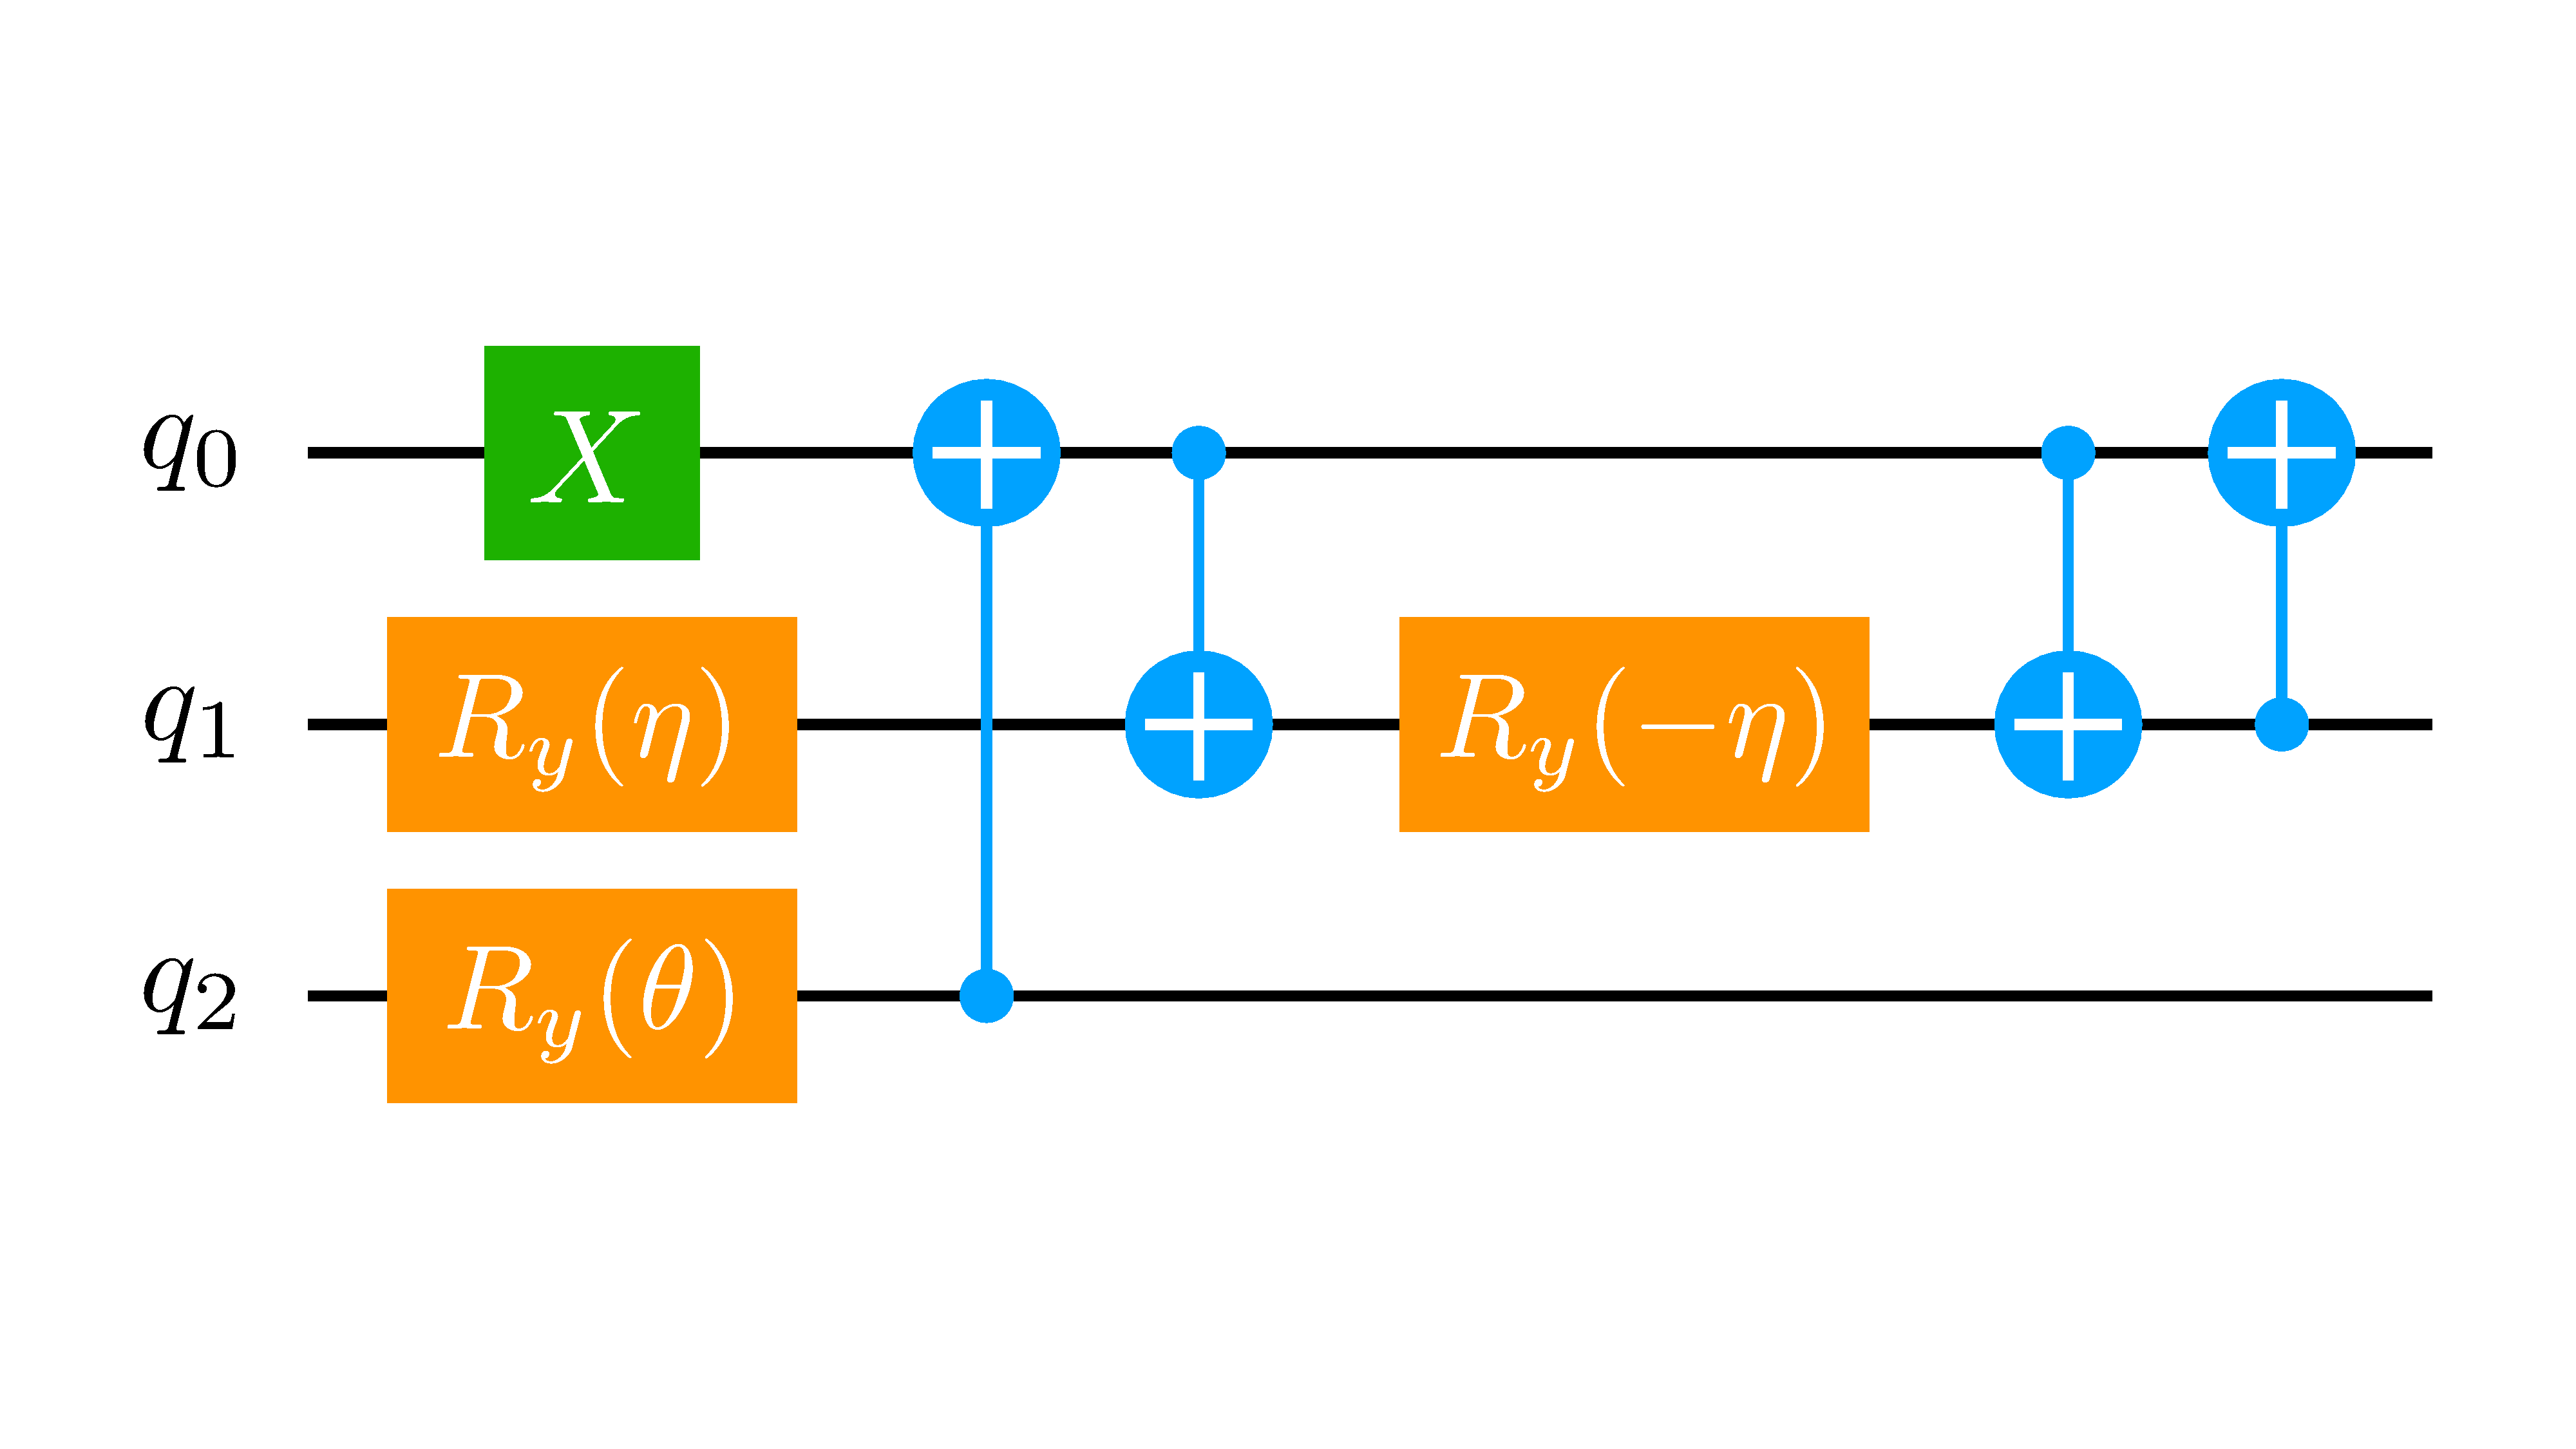
\includegraphics[width=.40\paperwidth]{Figures/chapter05/deuteron-quantum-circuits-2}
    \end{center}

  \end{multicols}

  \vspace{-1em}
  \begin{theorem}[Nyquist-Shannon]
    If a function $h(\theta)$ contains no angular frequencies higher than $\omega_{\textnormal{S}}$, it is completely determined by giving its ordinates at a series of points $1/2\omega_{\textnormal{S}}$ apart: $\omega_{\textnormal{sampling}} > 2\omega_{\textnormal{S}}$.
  \end{theorem}

\end{frame}

%% ----------------------------------------------------------------------------
%% ----------------------------------------------------------------------------

\subsection{Comparison}

\begin{frame}[allowframebreaks]{Algorithm comparison}

  \vspace{2em}
  \begin{itemize}
    \item Algorithmic complexity model:
  \end{itemize}
  \vspace{-2em}
  \begin{gather*}
    \frac{\textnormal{VQE}}{\textnormal{QSR}} = \qty(m n 2^{-n/r})^{p}
  \end{gather*}

  \vspace{-1em}
  \begin{multicols}{2}

    \begin{center}
      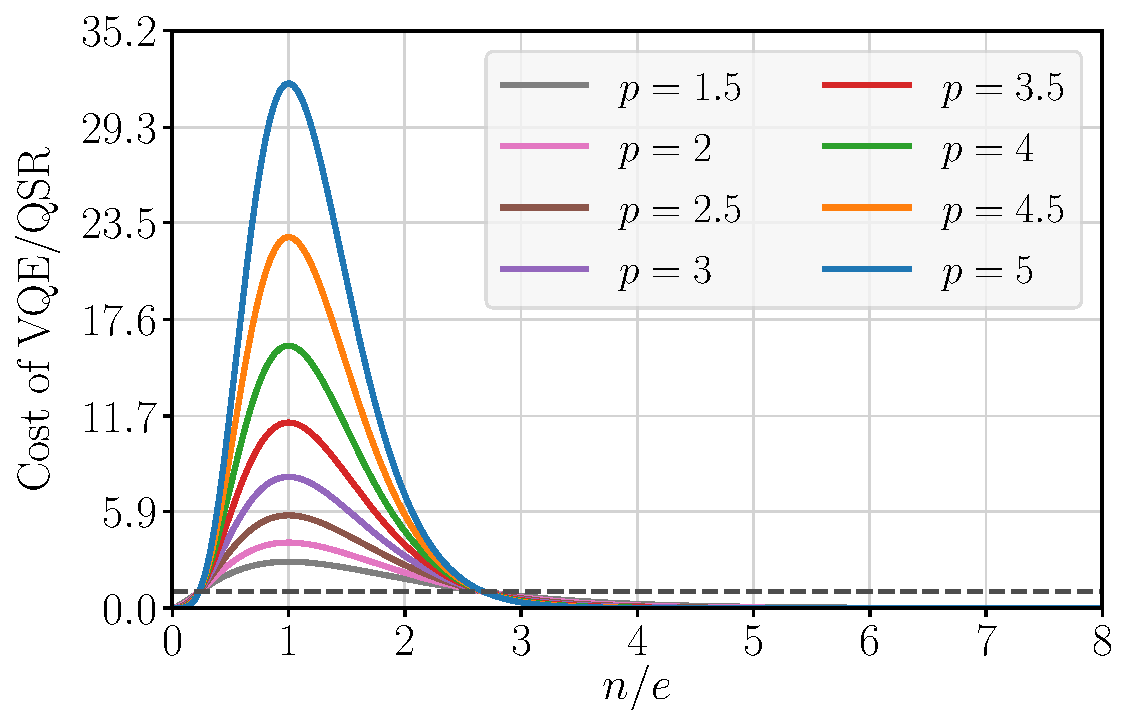
\includegraphics[width=.40\paperwidth]{Figures/chapter05/VQE-vs-QSR_p}
    \end{center}

    \columnbreak

    \begin{center}
      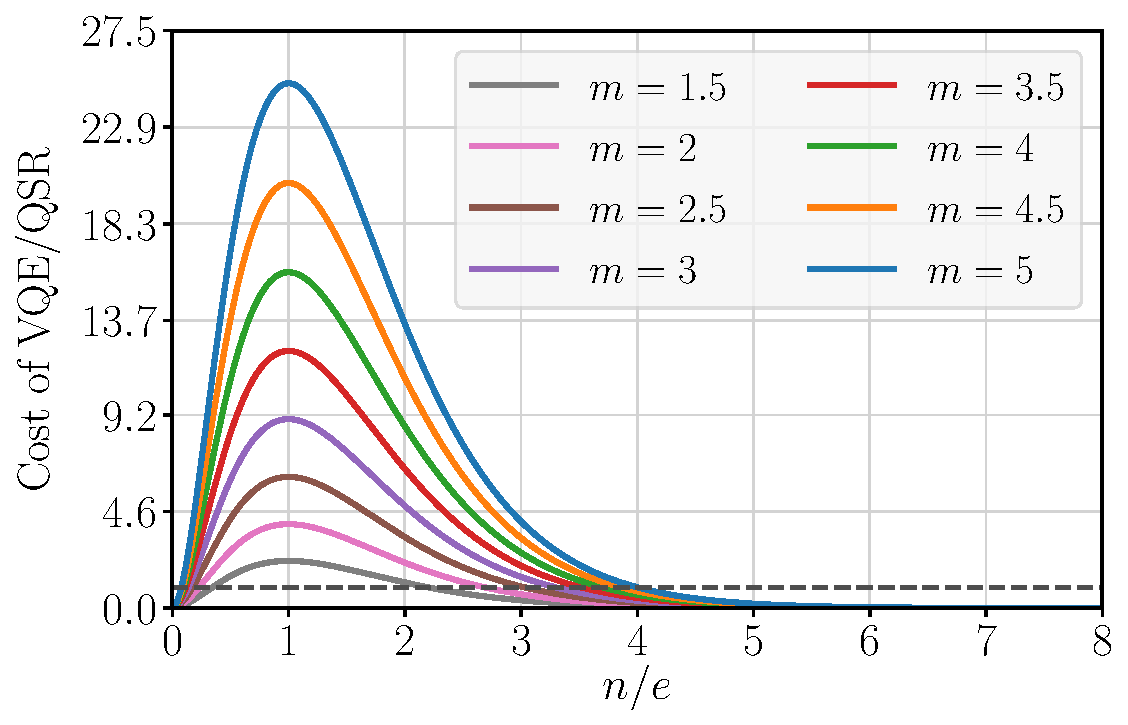
\includegraphics[width=.40\paperwidth]{Figures/chapter05/VQE-vs-QSR_m}
    \end{center}

  \end{multicols}

%% ----------------------------------------------------------------------------
\break
%% ----------------------------------------------------------------------------

  \begin{multicols}{2}

    \begin{center}
      Threshold \\
      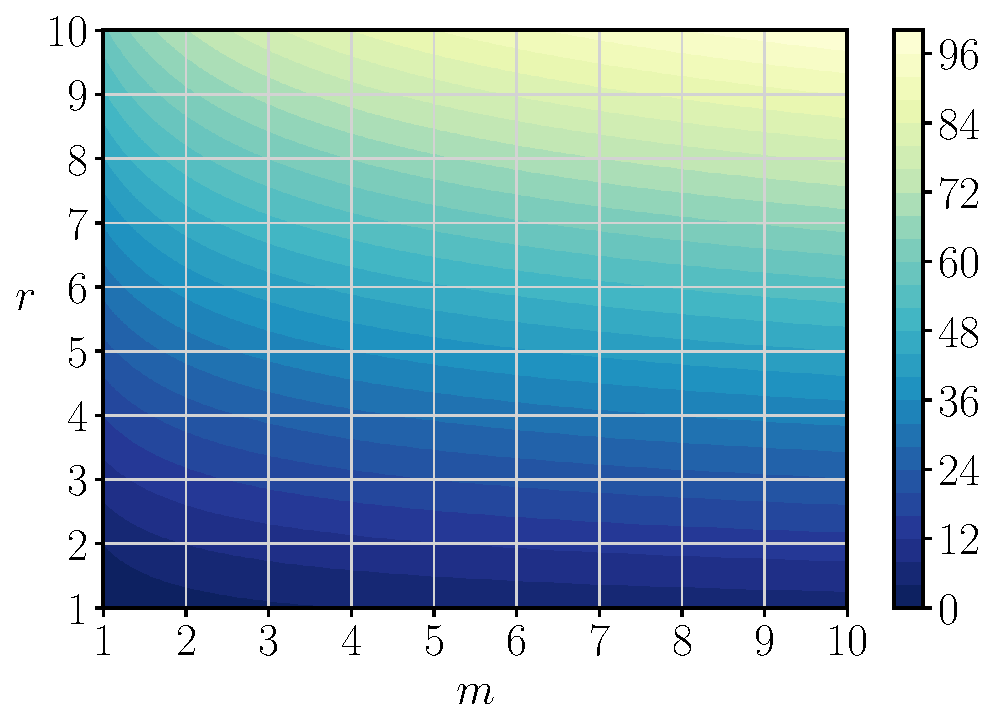
\includegraphics[width=.40\paperwidth]{Figures/chapter05/threshold}
    \end{center}

    \columnbreak

    \begin{center}
      Efficiency \\
      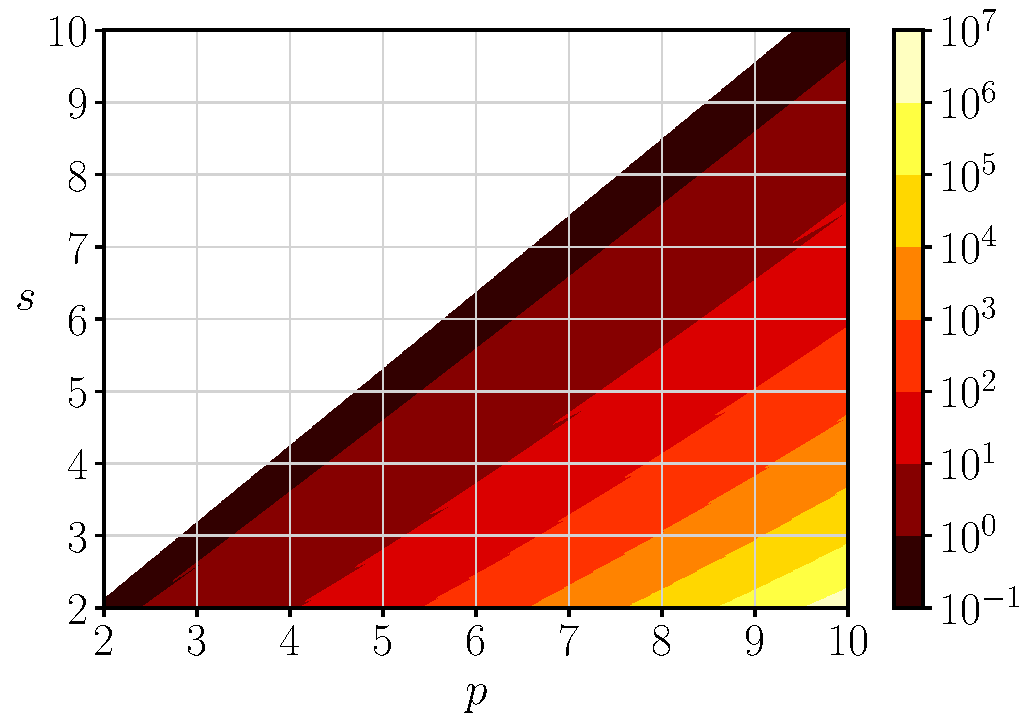
\includegraphics[width=.40\paperwidth]{Figures/chapter05/efficiency}
    \end{center}

  \end{multicols}
  \vspace{-3em}
  \begin{multicols}{2}

    \begin{gather*}
      a \defeq \ceil*{- \frac{r}{\ln{2}} W_{-1}\qty(-\frac{\ln{2}}{mr})}
    \end{gather*}

    \columnbreak

    \begin{gather*}
      E \approx \frac{1}{as\ln{2}} \qty(\frac{m}{s\ln{2}})^p
        \Gamma \qty(p+1, s\ln{2}, as\ln{2}) \label{eq:QSR-efficiency}
    \end{gather*}

  \end{multicols}

\end{frame}

%% ----------------------------------------------------------------------------
%% ----------------------------------------------------------------------------

\begin{frame}{Benchmark}

  \begin{figure}[!tbp]
  	\centering
  	\begin{minipage}[c]{.40\linewidth}
  		\centering
  		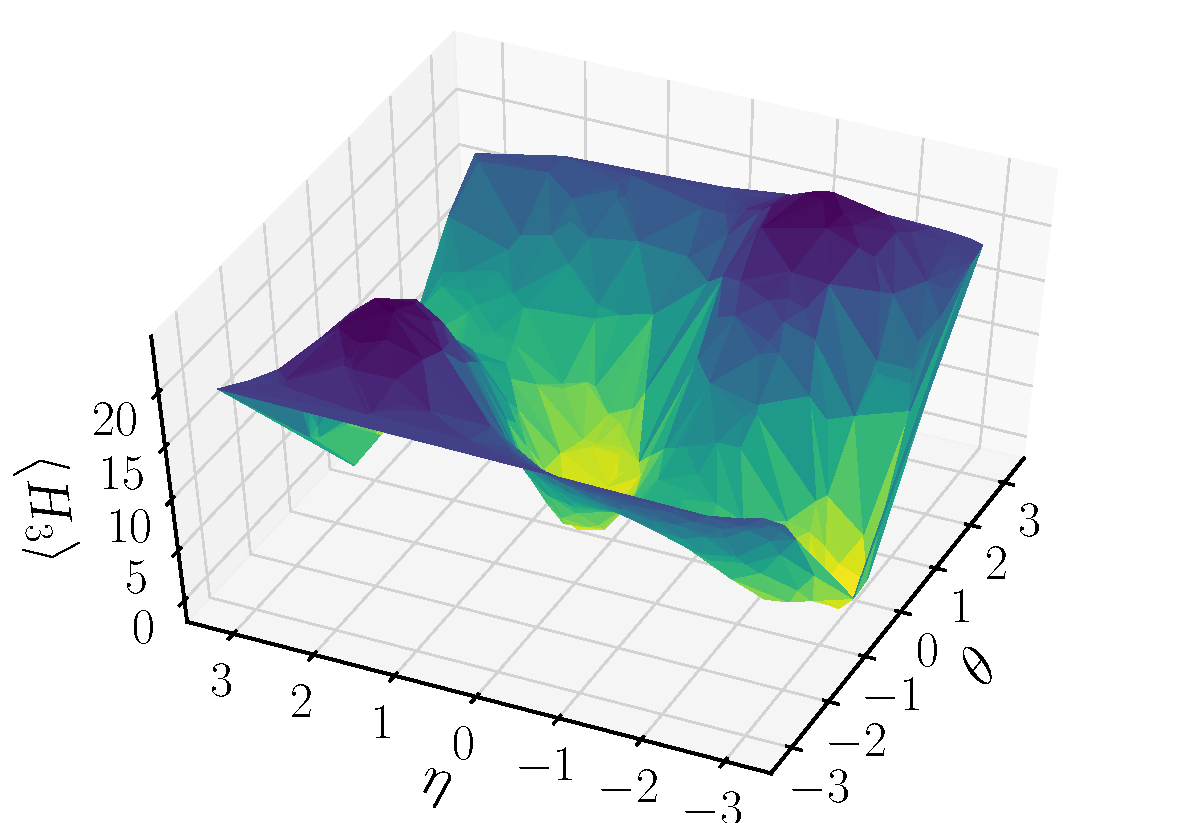
\includegraphics[width=\linewidth]{Figures/chapter05/deuteron-VQE}
  	\end{minipage}
  	\hspace{.025\linewidth}
  	\begin{minipage}[c]{.40\linewidth}
  		\centering
  		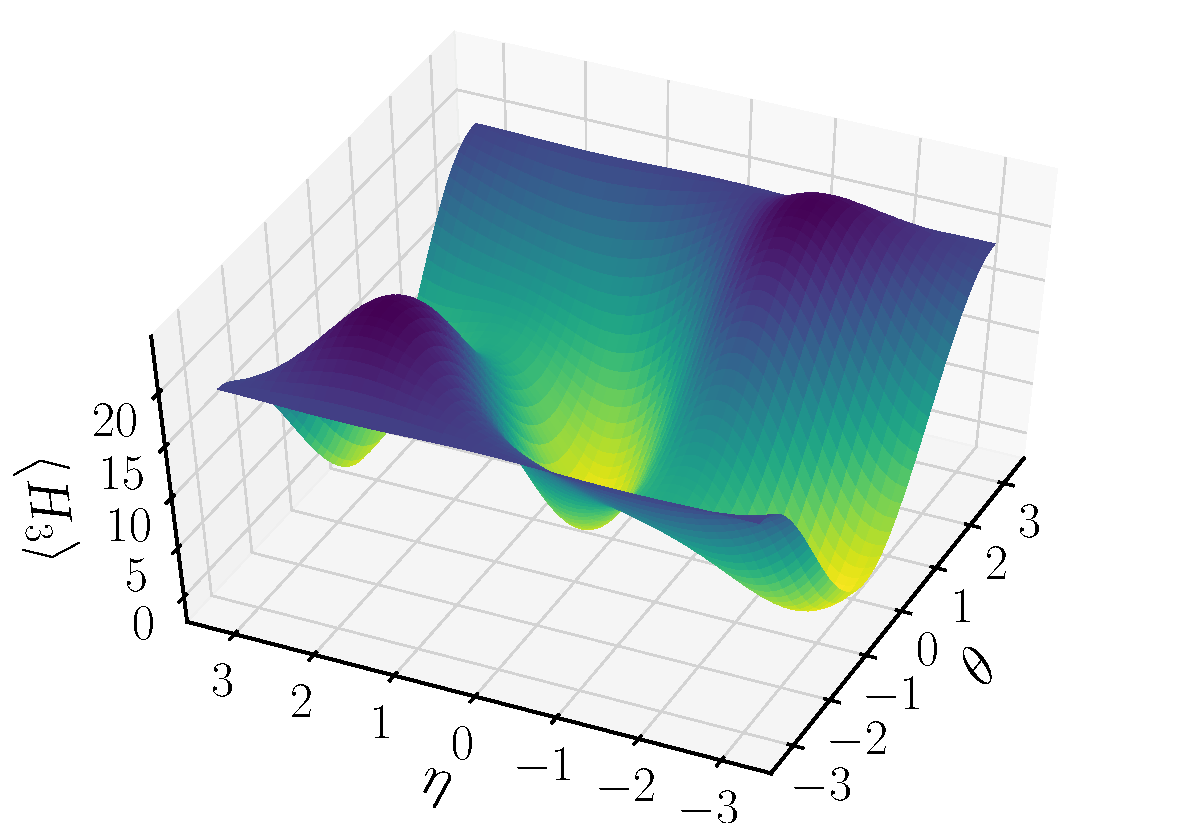
\includegraphics[width=\linewidth]{Figures/chapter05/deuteron-QSR}
  	\end{minipage}
  	\caption{Comparison between the VQE and QSR algorithms, when reproducing an external model with two parameters. (Left) Triangulation of the expectation value function from raw samples. (Right) Approximate function obtained through the Optimal Sampling Regression method with $S_q=S_{\text{max}}=2 ~\forall q$.}
  \end{figure}

  \vspace{-1em}

  \begin{table}[!bp]
  	\centering
  	% \caption{Comparison between results using the VQE and QSR algorithms.}
  	\begin{tabular}{ c c c c c }
  		\hline
  		\hline
  		$N_\text{params}$ & VQE samples & QSR samples &
  		VQE error & QSR error \\
  		\hline
  		$1$ & $24$ & $3$ & $3.5\%$ & $1.0\%$ \\
  		$2$ & $153$ & $25$ & $0.3\%$ & $0.2\%$ \\
  		\hline
  		\hline
  	\end{tabular}
  \end{table}

\end{frame}

%% ----------------------------------------------------------------------------
%% ----------------------------------------------------------------------------

\subsection{Applications}

%% ----------------------------------------------------------------------------
%% ----------------------------------------------------------------------------

\begin{frame}{Applications of QSR}

  \begin{multicols}{2}
    \begin{itemize}
      % \item \textbf{Reduce the amount of queries} necessary to solve a given optimization problem.
      \item \textbf{Oversampling} to attain higher precision.
      \item \textbf{Undersampling} to boost performance and get rid of small-wavelength oscillations leading to burdensome local minima.
      \item VQE low-resolution start-up \textbf{supplement}.
      \item \textbf{Proxy} to transition between simulators and real devices.
      \item Improve convergence by removing the stochastic nature of the quantum expectation value function.
      \item Avoid the exponential matrix formulation in classical computation.
    \end{itemize}

    \columnbreak

    \begin{center}
      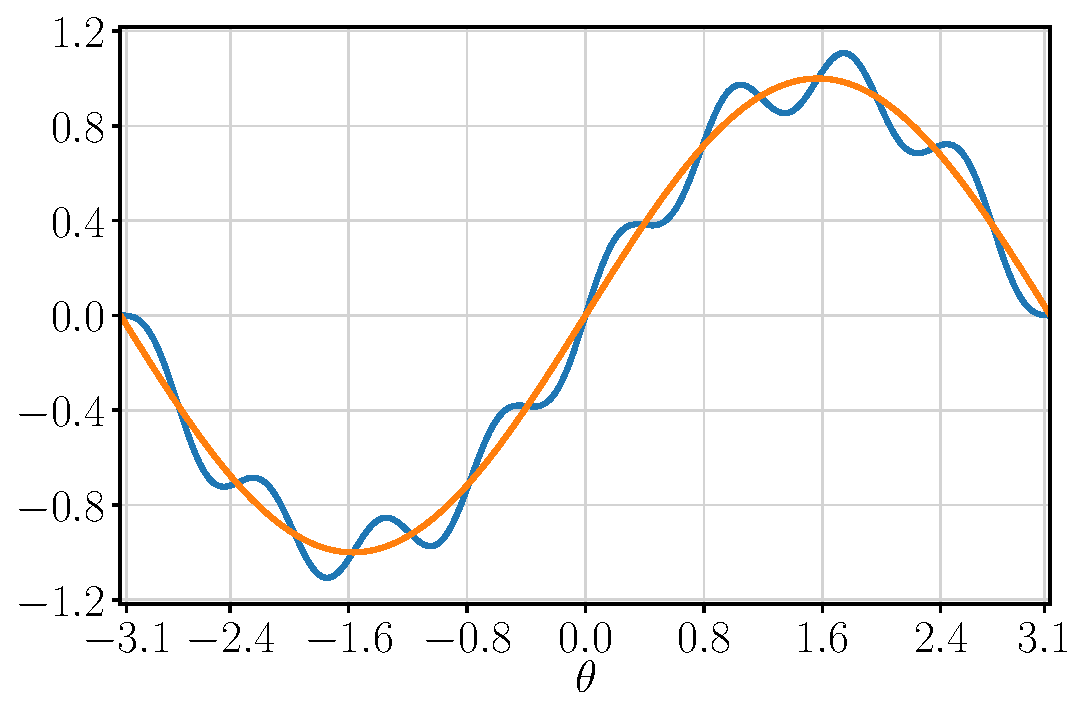
\includegraphics[width=.40\paperwidth]{Figures/low-resolution}
    \end{center}

  \end{multicols}

\end{frame}
